% This is samplepaper.tex, a sample chapter demonstrating the
% LLNCS macro package for Springer Computer Science proceedings;
% Version 2.20 of 2017/10/04
%
\documentclass[runningheads]{llncs}
%
\usepackage{graphicx}
\usepackage{amsfonts}
\usepackage{amsmath}

% Used for displaying a sample figure. If possible, figure files should
% be included in EPS format.
%
% If you use the hyperref package, please uncomment the following line
% to display URLs in blue roman font according to Springer's eBook style:
% \renewcommand\UrlFont{\color{blue}\rmfamily}

\begin{document}
%
\title{Multistage Global Search Using Various Scalarization Schemes in Multicriteria Optimization Problems\thanks{This research was supported by the Russian Science Foundation, project No 16-11-10150 ''Novel efficient methods and software tools for time-consuming decision making problems using supercomputers of superior performance.''}}
%
\titlerunning{Multistage Global Search in Multicriteria Optimization Problems}
% If the paper title is too long for the running head, you can set
% an abbreviated paper title here
%
\author{Victor Gergel\orcidID{0000-0002-4013-2329} \and
Evgeniy Kozinov\orcidID{0000-0001-6776-0096}}
%
\authorrunning{V. Gergel et al.}
% First names are abbreviated in the running head.
% If there are more than two authors, 'et al.' is used.
%
\institute{Lobachevsky State University of Nizhni Novgorod, Nizhni Novgorod, Russia
\email{gergel@unn.ru} \email{evgeny.kozinov@itmm.unn.ru}}
%
\maketitle              % typeset the header of the contribution
%
\begin{abstract}
In this paper, an approach, in which the decision making problems are reduced to solving the multicriteria time-consuming global optimization problems is proposed. The developed approach includes various methods of scalarization of the vector criteria, the dimensionality reduction with the use of the Peano space-filling curves and the efficient global search algorithms. In the course of computations, the optimization problem statements and the applied methods of the criteria scalarization can be altered in order to achieve more complete compliance to available requirements to the optimality. The overcoming of the computational complexity of the developed approach is provided by means of the reuse of the whole search information obtained in the course of computations. The performed numerical experiments have confirmed the reuse of the search information to allow reducing essentially the amount of computations for solving the global optimization problems.

\keywords{Decision making \and Multicriteria optimization \and Criteria scalarization \and Global optimization with nonlinear constraints \and Numerical experiment.}
\end{abstract}
%
%
%
\section{Introduction}	
\label{sec:01}
The multicriteria optimization (MCO) problems, which are used as the statements of the decision making problems often are the field of extensive research -- see, for example, the monographs \cite{c1,c2,c3} and the reviews of the scientific and applied results in this area \cite{c4,c5}.

Usually, the finding of the efficient (non-dominated) decisions, in which the improvement of the values with respect to any criteria cannot be achieved without the worsening of the values with respect to other criteria is understood as the solution of a MCO problem. In the most general case, when solving the MCO problems, it can appear to be necessary to obtain a complete set of the efficient decisions (the Pareto set). However, the finding of all efficient decisions may require a considerable amount of computations, and the set of obtained decisions may appear to be quite large. As a result, the approaches, which obtain the more limited set of efficient decisions are applied wider. Among such approaches, there are various kinds of the criteria convolutions, the lexicographic optimization methods, the algorithms of searching the best approximation to the given prototypes, etc. All methods mentioned above allow accounting for the specific features of the MCO problems being solved and satisfy the requirements to the optimality from the decision maker. 

The present work is devoted to the solving of the MCO problems, which are used for the description of the complex decision making problems, in which the criteria of efficiency may have a multiextremal form, and the determining of the values of the criteria and constraints may require a large amount of computations. Also, it was assumed that in the course of computations it is possible to change the problem statement, the methods, and the parameters of solving the MCO problem that results in the necessity of the multiple solving of the global optimization problems. 

The practical use of this approach implies the overcoming of a considerable computational complexity of the decision making problems that can be provided by means of the use of highly efficient global optimization methods and the complete utilization of the search information obtained in the course of computations.

In the present paper, the results of investigations on the generalization of the decision making problem statements \cite{c6,c7} and on the development of the highly efficient global optimization methods utilizing the whole search information obtained in the course of computations \cite{c8,c9,c10} are presented.

Further structure of the paper is as follows. In Section \ref{sec:02}, the statement of the decision making problems based on multistage multicriteria global optimization are presented. In Section \ref{sec:03}, a general scheme of the criteria scalarization is proposed. In Section \ref{sec:04}, the search information obtained in the course of computations is considered. In Section \ref{sec:05}, an efficient algorithm for solving the time-consuming global optimization problems with the nonlinear constraints is presented. Section \ref{sec:06} presents the results of numerical experiments confirming the developed approach to be promising. In Conclusion, the obtained results are discussed and possible main directions of further research are outlined.


\section{Multistage multicriteria optimization problem statement}	
\label{sec:02}
For the formal description of the process of solving the complex decision making problems, the following generalized two-phase scheme is proposed.

1.	In the most general form, a decision making problem is defined by means of a vector function of characteristics 
\begin{equation}\label{eq:1}
	w(y)=(w_1(y), w_2(y), \dots, w_M (y)), y \in D
\end{equation}
where $y=(y_1,y_2,\dots, y_N )$ is the vector of varied parameters and $D \subset R^N$ is the search domain, which is usually an $N$-dimensional hypercube
\begin{equation}\label{eq:2}
	D=\{y \in R^N:a_i \leq y_i \leq b_i,1 \leq i \leq N\}
\end{equation}
for given vectors $a$ and $b$. 

It is supposed, that the values of characteristics $w(y)$ are non-negative, and the decreasing of these ones corresponds to the increasing of the efficiency of the chosen decisions. Also, it is supposed that the characteristics $w_j (y)$, $1 \leq j \leq M$, may be multiextremal, and the determining of their values may require large enough amount of computations. Besides, the characteristics $w_j (y)$, $1 \leq j \leq M$, are supposed to satisfy the Lipschitz condition
\begin{equation}\label{eq:3}
	|w_j (y_1 )-w_j (y_2 )| \leq L_j \|y_1-y_2 \|, 1 \leq j \leq M
\end{equation}
where $L_j$ is the Lipschitz constant for the characteristic $w_j(y)$ , $1 \leq j \leq M$, and $\|*\|$ denotes the Euclidean norm in $R^N$. 

2.	Then, a MCO problem is formulated on the basis of the statement considered above. For this purpose, a vector criterion of efficiency is selected among the characteristics $w_j (y)$, $1 \leq j \leq M$, from (\ref{eq:1}) 
\begin{equation}\label{eq:4}
	f(y)=(f_1 (y),f_2 (y),\dots,f_s (y)), f_j (y)=w_{i_j} (y), 1\leq j \leq s, 1\leq i_j \leq M
\end{equation}
and the vector function of constraints
\begin{equation}\label{eq:5}
	g(y)=(g_1 (y),g_2 (y),\dots,g_m (y)), g_l (y)=w_{i_l} (y)-q_l, 1\leq l\leq m, 1 \leq i_l \leq M
\end{equation}
where $q_l>0$, $1 \leq l \leq m$, are the allowances on the feasible values of characteristics $w_j (y)$, $1 \leq j \leq M$.

The formulated criteria of efficiency and constraints allow to define a multicriteria optimization problem
\begin{equation}\label{eq:6}
	P : f(y)\to min, y \in Q
\end{equation}
where Q is the feasible search domain
\begin{equation}\label{eq:7}
	Q=\{ y\in D : g(y) \leq 0 \}.
\end{equation}

In development of this scheme of the MCO problem statement, further an opportunity of simultaneous formulation of several MCO problems 
\begin{equation}\label{eq:8}
	\mathbb{P}_t=\{ P_1,P_1,\dots,P_t \},
\end{equation}
will be allowed, the set of which can be varied in the course of computations by means of adding new or by removing already existing optimization problems. 

In general, the proposed scheme of the optimal decision search process (\ref{eq:1})-(\ref{eq:8}) defines a new class of the optimization problems -- the multistage multicriteria global optimization (MMGO) problems.

\section{Reduction of the multistage multicriteria search to the scalar one-dimensional global optimization problems}	
\label{sec:03}
One of the widely used approaches to solving the MCO problems is to transform the vector criterion into some general scalar criterion of efficiency that allows using a large set of already existing optimization methods for solving the global optimization problems. Among the possible scalarization methods, there are, for example, the weighted sum method, the compromise programming method, the weighted minimax method, and many other methods -- see, for example, \cite{c2,c3}. 

In the general form, the statement of the global optimization problems generated as a result the MCO problem criteria scalarization can be represented as follows:
\begin{equation}\label{eq:9}
	\min{\varphi(y) = F(\alpha,y)}, g(y) \leq 0, y \in D,
\end{equation}
where $F$ is the scalar objective function, $\alpha$ is the vector of parameters of the applied criteria scalarization method, $g(y)$ are the constraints of the MCO problem from (\ref{eq:6}), and $D$ is the search domain from (\ref{eq:2}).

Particular forms of the function $F(\alpha,y)$ are defined by the criteria scalarization methods applied. For example, the following scalarization methods are possible.

1.	In the case of equal importance of the criteria $f_i$, $1 \leq i \leq s$, the minimax convolution scheme (MMC) \cite{c3} can be applied:
\begin{equation}\label{eq:10}
\begin{split}
  F^1 (\lambda,y)=\max{⁡(\lambda_i f_i(y), 1 \leq i \leq s)},  \\
  \lambda=(\lambda_1,\lambda_2,\dots,\lambda_s) \in \Lambda \subset R^s:\sum_{i=1}^s{\lambda_i =1},\lambda_i \geq 0, 1 \leq i \leq s.
\end{split}
\end{equation}

2.	In the case of arrangement of the criteria in importance order, the method of successive concessions (MSC) \cite{c2,c3} can be used. In this case, the scalar objective function F can be set as follows
\begin{equation}\label{eq:11}
	\min F^2 (\lambda,y)=f_s (y),f_i (y) \leq f_i^{min}+\delta_i (f_i^{max}-f_i^{min} ),1 \leq i<s,g(y)\leq 0,y\in D,
\end{equation}
where $f_i^{min}$ and $f_i^{max}$ are the minimum and maximum values of the criteria $f_i (y)$, $1\leq i<s$, in the domain $D$ respectively, and $0 \leq \delta_i \leq 1$, $1\leq i<s$, are the concessions with respect to each criterion. As before, the values of concessions $0 \leq \delta_i\leq 1$, $1 \leq i<s$, can be varied in the course of computations. The quantities $f_i^{min}$ and $f_i^{max}$,  $1 \leq i<s$, the values of which may be unknown \textit{a priori}, can be replaced by the minimum and maximum estimates of the criteria values computed using the available search information.

3.	In the case of availability of any estimates of the criteria values of the required decision (for example, based on an ideal decision or on any existing prototype) the MCO problem solution may consist in finding an efficient decision the most completely matching given values of optimality (the reference point method, RPM). Such a problem can be formulated in the form of a scalar optimization problem
\begin{equation}\label{eq:12}
	\min{F^3 (\lambda,y) = 1 / s \sum_{i=1}^s{\theta_i (f_i (y)-f_i^* )^2 } },g(y)\leq 0,y \in D	
\end{equation}
where the objective function $F^3 (\lambda,y)$ is the standard deviation of the decision $y \in D$ from the sought ideal decision, and the quantities $0 \leq \theta_i \leq 1$, $1 \leq i<s$, are the magnitudes of importance of approximations with respect to each particular variable $y_i$, $1\leq i\leq N$.

Within the framework of the developed approach, it is possible to change the used scalarization methods (\ref{eq:10})-(\ref{eq:12}) and/or altering the parameters of convolutions $\lambda$, $\delta$ and $\theta$. Such variations expand the set of the MCO problems $\mathbb{P}$ from (\ref{eq:8}) necessary for solving the initial decision making problem into a wider set of the scalar global optimization problems (\ref{eq:9})
\begin{equation}\label{eq:13}
	\mathbb{F}_T=\{ F_i (\alpha_i,y): 1\leq i \leq T \},
\end{equation}
in which each problem $P\in \mathbb{P}$ from (\ref{eq:8}) can correspond to several global optimization problems (\ref{eq:9}).

In the developed approach, one more step of converting the problems being solved $F(\lambda,y)$ from (\ref{eq:9}) is applied, namely the dimensionality reduction is performed with the use of the Peano space-filling curves (evolvents) $y(x)$ providing an unambiguous mapping of the interval [0,1] onto an $N$-dimensional hypercube $D$ \cite{c11,c12}. As a result of such reduction, the multidimensional global optimization problem (\ref{eq:9}) is reduced to a one-dimensional problem
\begin{equation}\label{eq:14}
	F(\alpha,y(x^* ))=\min{\{ F(\alpha,y(x)) : g(y(x))\leq 0, x\in[0,1] \}.}
\end{equation}

The dimensionality reduction allows applying many well known highly efficient one-dimensional global optimization algorithms for solving the problems (\ref{eq:9}) (after performing necessary generalization) -- see, for example, \cite{c11,c12,c13,c14,c15}.


\section{Computational complexity reduction of the multistage multicriteria search on the basis of the reuse of the search information}	
\label{sec:04}

The numerical solving of the global optimization problems (\ref{eq:9}) is usually implemented by the successive computing the values of characteristics $w(y)$ at the points $y^i$, $0\leq i\leq k$, of the search domain $D$ \cite{c11,c14}. The data obtained as a result of computations can be represented in the form of the matrix of the search information
\begin{equation}\label{eq:15}
	\Omega_k=\{ (y^i,w^i=w(y^i ))^T: 1\leq i \leq k \}.
\end{equation}

As a result of scalarization (\ref{eq:9}) and the use of the dimensionality reduction (\ref{eq:14}), the set $\Omega_k$ from (\ref{eq:15}) can be transformed into the form of the matrix of the search state
\begin{equation}\label{eq:16}
	A_k={ (x_i,z_i,g_i,l_i )^T: 1\leq i \leq k },
\end{equation}
where $x_i$, $1\leq i\leq k$, are the reduced points of the executed global search iterations, $z_i$, $g_i$, $1\leq i\leq k$, are the values of the scalar criterion and constraints of current optimization problem $F(\alpha,y(x))$ at these points, and $l_i$, $1\leq i\leq k$, are the indices of global search iterations, in which the points $x_i$, $1\leq i\leq k$, were computed.

The availability of the set $\Omega_k$ from (\ref{eq:15}) allows reducing the results of all preceding computations $z_i$, $1\leq i\leq k$ from the matrix $A_k$ to the values of the next optimization problem $F(\alpha,y(x))$ from (\ref{eq:9}) without any repeated time-consuming computations of the values of $w(y)$ from (\ref{eq:1}), i. e.
\begin{equation}\label{eq:17}
	w_i \xrightarrow{\alpha,P} (z_i,g_i ), 1\leq i\leq k, \forall \alpha, P\in \mathbb{P}
\end{equation}

The reuse of the search information can provide a gradual decreasing of the amount of computations when solving every next optimization problem down to the execution of few iterations only to find the next efficient decision.

\section{Efficient solving the multistage multicriteria optimization problems with nonlinear constraints}	
\label{sec:05}
Within the framework of developed approach, the efficient method was applied for solving the global optimization problems with the nonlinear constraints \cite{c11}. The essence of the approach is the constructing of a problem with some aggregated unconstrained objective function, the solving of which leads to the solution of the initial problem (\ref{eq:9}) -- more detailed description of the approach will be given below.

Let us introduced a simpler notation for the reduced problems (\ref{eq:14}) as
\begin{equation}\label{eq:18}
%\begin{split}
	\min{\{g_{m+1} (x):g_i (y(x)) \leq 0, 1\leq i \leq m,x \in [0,1]\} }, g_{m+1} (x)=F(\lambda,y(x)).
%\end{split}
\end{equation}

The problem (\ref{eq:18}) can be considered in the statement of partial computability when each function $g_j (y)$, $1 \leq j \leq m+1$ is defined and computable in certain subinterval $\Delta_j \subset [0,1]$ only where
\begin{equation}\label{eq:19}
	\Delta_1=[0,1], \Delta_{j+1}=\{ x \in \Delta_j  : g_j (y(x))\leq 0 \}, 1\leq j\leq m.
\end{equation}

Taking into account the conditions (\ref{eq:19}), the objective function of the problem (\ref{eq:18}) can be represented in the form 
\begin{equation}\label{eq:20}
	\varphi(x^*)=\min{\{ g_{m+1} (y(x)) : x\in \Delta_{m+1} \}},
\end{equation}
on the basis of which the problem (\ref{eq:18}) can be transform to the problem of minimizing the aggregated function 
\begin{equation}\label{eq:21}
\begin{split}
	\min{\{ \Phi(y(x))=g_v(y(x)), v=v(x), x\in[0,1] \}}, \\	
	1\leq v=v(x)\leq m+1, g_v (y(x))>0, g_j (y(x))\leq 0, 1\leq j\leq v-1.
\end{split}
\end{equation}

The index $v=v(x)$, $1\leq v \leq m+1$ defines the first violated constraint at the point $x$ in successive calculation of constraints.

Within the framework of the developed approach, the algorithm of global constrained optimization (AGCO), which is considered in details in \cite{c11} is applied for solving the global unconstrained problems (\ref{eq:21}).



\section{Results of numerical experiments}	
\label{sec:06}
The numerical experiments have been carried out using the computational nodes of Lobachevsky supercomputer at Nizhni Novgorod State University. The peak performance of the supercomputer was 573 Tflops, each computational node was equipped with Intel Sandy Bridge E5-2660 processor 2.2 GHz, 64 Gb RAM. 

Within the framework of the present paper, the construction of a numerical approximation (PDA) of the Pareto domain (PD) was understood as a solution of a MCO problem. In order to evaluate the efficiency of constructing the PDA, two main indicators applied widely were used: the completeness of coverage of the Pareto domain (hypervolume index, HV) and the uniformity of distribution of the numerical estimates of the efficient decisions (distribution uniformity index, DU) \cite{c10}. The higher values of the index HV and the lower values of the index DU corresponds to the better approximation. 

Within the executed experiments, the two-dimensional bi-criterial MCO problems were used, the criteria of which were defined with the use of the family of multiextremal functions \cite{c11}. The functions of this family are defined as follows
\begin{equation}\label{eq:22}
\begin{split}
f(y_1,y_2 )= -(AB+AC)^{1/2},\\
AB=(\sum_{i=1}^7 {\sum_{j=1}^7{[A_{ij} a_{ij} (y_1,y_2 )+B_{ij} b_{ij} (y_1,y_2 )]}} )^2,\\
CD=(\sum_{i=1}^7 {\sum_{j=1}^7{[C_{ij} a_{ij} (y_1,y_2 )-D_{ij} b_{ij} (y_1,y_2 )]}} )^2,
\end{split}
\end{equation}
where the expressions 
\begin{equation*}
	a_{ij} (y_1, y_2)=sin(\pi iy_1 )  sin(\pi jy_2 ), b_{ij} (y_1,y_2 )=cos(\pi iy_1 ) cos(\pi jy_2 )
\end{equation*}
are defined in the area $0\leq y_1,y_2\leq 1$, and the parameters $-1 \leq A_{ij},B_{ij},C_{ij},D_{ij} \leq 1$ are the independent random numbers distributed uniformly in the same interval.

The initial series of the numerical experiments was performed to evaluate the positive effect (the reducing of the number of the executed iterations) due to the reuse of the search information obtained in the course of computations (see Section \ref{sec:04}). When conducting the experiments, the AGCO algorithm was applied sequentially with all scalarization methods considered in Section Section \ref{sec:03}: the minimax convolution of the criteria (\ref{eq:10}), the method of successive concessions (\ref{eq:11}), and the reference point method (\ref{eq:12}). For each method mentioned above, 50 subproblems with various values of the parameters $\lambda$, $\delta$ and $\theta$ correspondingly have been solved. In order to evaluate the indicator HV of the completeness of the PDA approximation, the reference point (-4,-4) was used. For the AGCO algorithms, the reliability parameter $r=2.3$ was used; the accuracy in the stopping condition was set as $\varepsilon=0.01$.

The results of performed experiments are presented in Table 1. The column ''Iters'' contains the total number of iterations (the number of computations of the criteria values) required for solving the problem (\ref{eq:22}). The column ''PDA'' shows the number of the obtained efficient decisions in the PDA. In the first part of the table (columns 2-5), the results of solving all subproblems without the use of the search information are shown. In the second part (columns 6-9) the results of solving the same subproblems but with the use of the whole search information obtained in the course of computations (i. e. when solving every next subproblem, the search information obtained when solving all preceding subproblems was utilized) are presented. In the column ''S'', the speedup obtained as a result of reducing the number of the global search iterations (the number of the computed criteria values) required to solve all 50 subproblems due to the reuse of the search information is shown.

The results of experiments presented in Table 1 demonstrate the reduction of the number of the executed iterations of the AGCO algorithm more than 9 times. At that, the indicator HV takes almost the same values independently on the usage of the search information. However, the indicator DU was better notably (except the method of successive concessions) at the computations without the use of the search information (similar remark can be expressed on the number of efficient decisions in the PDA as well) -- most likely, this effect is manifested due to essentially less number of the executed iterations when using the search information. One can note also that the reference point method has some advantage in the efficiency indicators (the number of points in PDA, indicators HV and DU). However, this method inferior the use of the minimax convolutions in the number of iterations required to solve all 50 subproblems essentially.

\begin{table}[t]
\centering
\caption{Efficiency of the reuse of the search information in solving the problem (\ref{eq:22}) using various criteria scalarization methods}
\label{tab:01}
\begin{tabular}{ccccclcccclc}
\hline
              & \multicolumn{9}{c}{Search information}                      &  &     \\ \cline{2-10}
Scalarization & \multicolumn{4}{c}{Not used} &  & \multicolumn{4}{c}{Used}  &  & S   \\ \cline{2-5} \cline{7-10}
method        & Iters  & PDA  & HV    & DU   &  & Iters & PDA & HV   & DU   &  &     \\ \cline{1-5} \cline{7-10} \cline{12-12} 
MMC (\ref{eq:10})      & 9124   & 152  & 53.4  & 0.64 &  & 922   & 44  & 52.7 & 0.91 &  & 9.9 \\
MSC (\ref{eq:11})      & 12802  & 88   & 52.8  & 1.16 &  & 1402  & 40  & 52.4 & 1.09 &  & 9.1 \\
RPM (\ref{eq:12})      & 12881  & 240  & 53.6  & 0.51 &  & 1323  & 56  & 53.0 & 0.83 &  & 9.7 \\ \hline
\end{tabular}
\end{table}

In the last experiment, solving a test MCO problem has been conducted with a use of the search information but the applied criteria scalarization methods varied in the course of computations. In this experiment, at the first stage of computations, the minimax criteria convolution was used in solving three subproblems (\ref{eq:10}) with the convolution coefficients (1,0), (0.5,0.5), and (0,1), correspondingly. At the second stage, the scalarization method was changed to the reference point method (12), where the estimate (-14,-7) was used as the reference point with the weighting coefficients (0.5,0.5). And finally, at the third stage, the method of successive concessions (\ref{eq:11}) was applied with the concession with respect to the first criterion $\delta=0.5$.

\begin{table}[ht]
\centering
\caption{Results of solving the problem (\ref{eq:22}) with altering the criteria scalarization methods in the course of computations}
\label{tab:02}
\begin{tabular}{lccc}
\hline
Stage of computations, criteria scalarization method & Total iters & New iters & PDA \\ \hline
1. MMC (10), three subproblems                       & 304         & 304       & 14  \\
2. RPM (12)                                          & 402         & 98        & 19  \\
3. MSC (11)                                          & 437         & 35        & 24  \\ \hline
\end{tabular}
\end{table}

The results of performed experiments are given in Table 2. The column ''Total iters'' contains the total number of executed global search iterations whereas the column ''New iters'' shows the points of iterations executed at particular stage of solving the problem only. As follows from the results presented in Table 2, the number of the global search iterations executed at separate stages of solving the MCO is continuously problem reduced (from 304 down to 35), and the reuse of the search information provides the computationally efficient opportunity for dynamic variations of the criteria scalarization methods applied in the course of the MCO problem solution.


The PDA approximations of Pareto set obtained at the sequentially executed stages are shown in Fig. 1.
\begin{figure}[ht]
	\centering
		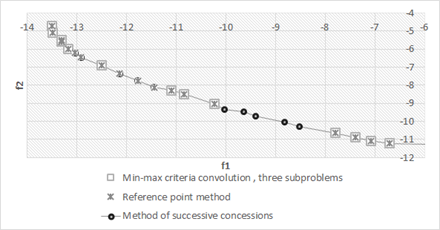
\includegraphics[width=0.70\textwidth]{fig1}
	\caption{Approximations of the Pareto set PDA obtained at the sequentially executed stages of computations}
	\label{fig:1}
\end{figure}

\section{Conclusion}
An approach is proposed to transform the decision making problems to the multi-stage multicriteria time-consuming global optimization problems. As a key property of the proposed approach it is supposed that the optimization problem statements and the applied methods of the criteria scalarization can be changed in the course of computations. The computational complexity is reduced by means of the reuse of the computed search information. The performed numerical experiments have confirmed the developed approach is promising.

In further investigations it is intended to execute the numerical experiments on solving the problems for a larger number of efficiency criteria and for larger dimensionality. Parallel computations can be considered as well.


%
% ---- Bibliography ----
%
% BibTeX users should specify bibliography style 'splncs04'.
% References will then be sorted and formatted in the correct style.
%
% \bibliographystyle{splncs04}
% \bibliography{mybibliography}
%
\begin{thebibliography}{8}

\bibitem{c1}	Parnell, G.S., Driscoll, P.J., Henderson, D.L., editors.: Decision Making in Systems Engineering and Management. Wiley, New Jersey (2008).
\bibitem{c2}	Collette, Y., Siarry, P.: Multiobjective Optimization: Principles and Case Studies (Decision Engineering). Springer. (2011).
\bibitem{c3}	Pardalos, P.M., {\v Z}ilinskas, A., {\v Z}ilinskas, J.: Non-Convex Multi-Objective Optimization. Springer. (2017).
\bibitem{c4}	Hillermeier, C., Jahn, J.: Multiobjective optimization: survey of methods and industrial applications. Surv. Math. Ind. \textbf{11}, 1--42 (2005).
\bibitem{c5}	Modorskii, V.Y., Gaynutdinova, D.F., Gergel, V.P., Barkalov, K.A.: Optimization in design of scientific products for purposes of cavitation problems. AIP Conference Proceedings, \textbf{1738}, 400013 (2016). \doi{10.1063/1.4952201}
\bibitem{c6}	Strongin, R.G., Gergel, V.P.: Parallel computing for globally optimal decision making. Lecture Notes in Computer Science, \textbf{2763}, 76--88 (2003).
\bibitem{c7}	Gergel, V.P., Kozinov, E.A.: Accelerating multicriterial optimization by the intensive exploitation of accumulated search data. AIP Conference Proceedings, \textbf{1776}, 090003 (2016). \doi{10.1063/1.4965367}
\bibitem{c8}	Gergel, V.: An Unified Approach to Use of Coprocessors of Various Types for Solving Global Optimization Problems. 2nd International Conference on Mathematics and Computers in Sciences and in Industry. (2015). \doi{10.1109/MCSI.2015.18}
\bibitem{c9}	Barkalov, K., Gergel, V., Lebedev, I.: Solving global optimization problems on GPU cluster. AIP Conference Proceedings, \textbf{1738}, 400006 (2016). \doi{10.1063/1.4952194}
\bibitem{c10}	Gergel, V.P., Kozinov, E.A.: Efficient multicriterial optimization based on intensive reuse of search information. J Glob Optim. \textbf{71}(1), 73--90 (2018). \doi{10.1007/s10898-018-0624-3}
\bibitem{c11}	Strongin, R., Sergeyev, Ya.: Global optimization with non-convex constraints. Sequential and parallel algorithms. Kluwer Academic Publishers, Dordrecht (2nd ed. 2013, 3rd ed. 2014).
\bibitem{c12}	Sergeyev Y.D., Strongin R.G., Lera D.: Introduction to global optimization exploiting space-filling curves. Springer. (2013).
\bibitem{c13}	Zhigljavsky, A., {\v Z}ilinskas, A.: Stochastic Global Optimization. Springer, Berlin. (2008).
\bibitem{c14}	Locatelli, M., Schoen, F. Global Optimization: Theory, Algorithms, and Applications. SIAM. (2013).
\bibitem{c15}	Floudas, C.A., Pardalos, M.P.: Recent Advances in Global Optimization. Princeton Univer-sity Press. (2016).



\end{thebibliography}
\end{document}
